\documentclass[student]{LSRslides}

\addbibresource{ref.bib}
\graphicspath{{pics/}{logos/}}

\title{Titel der Präsentation}
\presenter{S. Student}

\supervisor{B. Betreuer}
\typeofpres{Zwischenbericht Diplomarbeit}



%%%%%%%%%%%%%%%%%%%%%%%%%%%%%%%%%%%%%%%%%%%%%%%%%%%%%%%%%%%%%%%%%%%%%%%%%%%%%%%%

\begin{document}


\begin{frame}
    \titlepage
\end{frame}

\begin{frame}
    \frametitle{Übersicht}
    \tableofcontents%[hideallsubsections]%[pausesections]
\end{frame}

\section{Einführung}

\begin{frame}
	\frametitle{Einführung1}
	\begin{itemize}
 		\item $y=x^2+\sqrt{z}+\int_{a}^{b}{xyz}$
	\end{itemize}
\end{frame}

\begin{frame}
	\frametitle{Einführung2}

%\begin{figure}[htb]
%\centering
%\psfrag{q1}[Bl][Bl]{\small $\alpha$}
%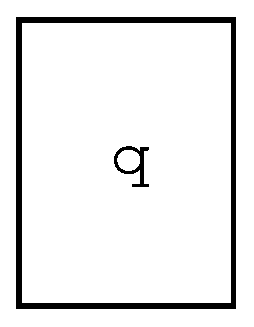
\includegraphics[width=0.9\textwidth]{samplefigure.eps}
%\caption{Sample Figure}
%\end{figure}

\end{frame}

\begin{frame}
	\frametitle{Related Work}
	Normal cite: \cite{buss11}\\
	Bigger cite: \scite{buss11}\\
	Variable number of authors: 
	\begin{itemize}
		\item 2 authors: \varcite{bauer09}{2}
		\item 4 authors: \varcite{bauer09}{4}
	\end{itemize}
\end{frame}

\section{Methoden}

\begin{frame}
	\frametitle{Methoden1}
	\begin{itemize}
		\item a
		\item b
	\end{itemize}
\end{frame}

\begin{frame}
	\frametitle{Methoden2}
	\begin{itemize}
		\item a
	\end{itemize}
\end{frame}

\begin{frame}
	\frametitle{Methoden3}
	\begin{itemize}
		\item a
	\end{itemize}
\end{frame}

\section{Ergebnisse}

\begin{frame}
	\frametitle{Ergbenisse1}
	...
\end{frame}

\begin{frame}
	\frametitle{Ergebnisse2}
	...
\end{frame}

\section{Zusammenfassung}

\begin{frame}
	\frametitle{Zusammenfassung}
	...
\end{frame}
\appendix
%\nocite{buss11}
%\nocite{bauer09}
\begin{frame}
	\frametitle{References}
	%\tiny
	%\bibliographystyle{plain}
	%\bibliography{ref}
	\printbibliography
\end{frame}


\end{document}
